\mySection{12.2 The $F$ Test}
%-------------- start slide -------------------------------%{{{ 12.13
\begin{frame}
	% {\S\: 12.2 The $F$ Test}
	\begin{minipage}{0.6\textwidth}
	\begin{enumerate}
		\item[] {\bf Model assumptions}
		\item Independence of observations
		\item Normality
		\item Homogeneity of variances
	\end{enumerate}
	\end{minipage}\pause
	\begin{minipage}{0.38\textwidth}
		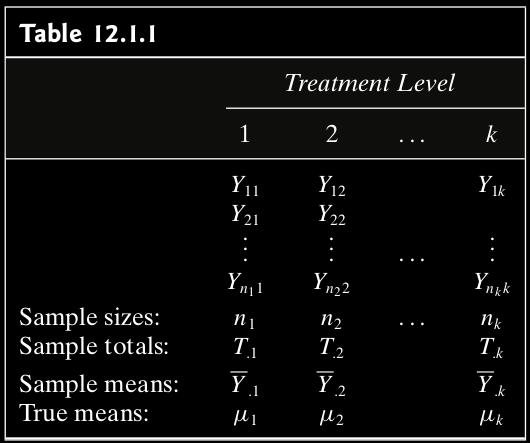
\includegraphics[scale=0.2]{Table_12-1-1-neg.png}
	\end{minipage}
\vfill

			\begin{minipage}{0.4\textwidth}
			\[\Updownarrow\]
			\end{minipage}
\vfill

	\begin{minipage}{0.4\textwidth}
		{\noindent\bf Assume:} \\
		$\forall j=1,\cdots, k$, $\forall j=1,\cdots, n_i$,
	\begin{enumerate}
		\item $Y_{ij}$ are independent.
		\item $Y_{ij}\sim N(\mu_j,\sigma^2)$
	\end{enumerate}
	\end{minipage}\pause
	\hfill $\Longleftrightarrow$ \hfill
	\begin{minipage}{0.45\textwidth}
		{\noindent\bf Assume:} \\
		$\forall j=1,\cdots, k$, $\forall j=1,\cdots, n_i$,\\
		\phantom{aaaaa} $Y_{ij} = \mu_j + \epsilon_{ij}$
	\begin{enumerate}
		\item $\epsilon_{ij}$ are independent.
		\item $\epsilon_{ij}\sim N(0,\sigma^2)$
	\end{enumerate}
	\end{minipage}
\end{frame}
%-------------- end slide -------------------------------%}}}
%-------------- start slide -------------------------------%{{{ 12.14
\begin{frame}[fragile]{Likelihood ratio test}

	\begin{enumerate}
		\item The parameter spaces are
			\[
				\Omega = \left\{
					(\mu_1,\cdots,\mu_k,\sigma^2):\:-\infty< \mu_1\alert{,\cdots,}\mu_k<\infty, \sigma^2>0
				\right\}
			\]
		\item[]
			\[
				\omega = \left\{
					(\mu_1,\cdots,\mu_k,\sigma^2):\: -\infty<\mu_1\alert{=\cdots=}\mu_k<\infty, \sigma^2>0
				\right\}
			\]
			\vfill
		\item The likelihood functions are
			\[
				L(\omega) = \left(  \frac{1}{2\pi\sigma^2}\right)^{n/2} \exp\left\{- \frac{1}{2\sigma^2}\sum_{j=1}^k\sum_{i=1}^{n_j}(y_{ij}-\alert{\mu})^2 \right\}
			\]
		\item[]
			\[
				L(\Omega) = \left(  \frac{1}{2\pi\sigma^2}\right)^{n/2} \exp\left\{- \frac{1}{2\sigma^2}\sum_{j=1}^k\sum_{i=1}^{n_j}(y_{ij}-\alert{\mu_j})^2 \right\}
			\]
	\end{enumerate}
\end{frame}
%-------------- end slide -------------------------------%}}}
%-------------- start slide -------------------------------%{{{ 12.15
\begin{frame}[fragile]

	\begin{enumerate}
		\setcounter{enumi}{2}
		\item Now
			\[
				\frac{\partial\ln L(\omega)}{\partial \mu} = \frac{1}{\sigma^2}\sum_{j=1}^k\sum_{i=1}^{n_j}(y_{ij}-\alert{\mu})
			\]
		\item[]
			\[
				\frac{\partial\ln L(\omega)}{\partial (\sigma^2)} = -\frac{n}{2\sigma^2} + \frac{1}{2\sigma^4}\sum_{j=1}^k\sum_{i=1}^{n_j}(y_{ij}-\alert{\mu})^2
			\]
			\vfill
		\item[] Setting the above derivatives to zero, the solutsions for $\mu$ and $\sigma^2$ are,
			\vfill
			\begin{align*}
				\frac 1n \sum_{j=1}^k\sum_{i=1}^{n_j} y_{ij} &= \bar{y}_{\cdot\cdot}\\
				\frac 1n \sum_{j=1}^k\sum_{i=1}^{n_j} (y_{ij}-\bar{y}_{\cdot\cdot})^2 &=v
			\end{align*}
	\end{enumerate}
\end{frame}
%-------------- end slide -------------------------------%}}}
%-------------- start slide -------------------------------%{{{ 12.16
\begin{frame}[fragile]

	\begin{enumerate}
		\item[3'] Similarly,
			\[
				\frac{\partial\ln L(\Omega)}{\partial \mu_j} = \frac{1}{\sigma^2}\sum_{j=1}^k\sum_{i=1}^{n_j}(y_{ij}-\alert{\mu_j}),\quad j=1,\cdots,k
			\]
		\item[]
			\[
				\frac{\partial\ln L(\Omega)}{\partial (\sigma^2)} = -\frac{n}{2\sigma^2} + \frac{1}{2\sigma^4}\sum_{j=1}^k\sum_{i=1}^{n_j}(y_{ij}-\alert{\mu_j})^2
			\]
			\vfill
		\item[] Setting the above derivatives to zero, the solutsions for $\mu_j$ and $\sigma^2$ are,
			\vfill
			\begin{align*}
				\frac{1}{n_j} \sum_{i=1}^{n_j} y_{ij} &= \bar{y}_{\cdot j}\\
				\frac 1n \sum_{j=1}^k\sum_{i=1}^{n_j} (y_{ij}-\bar{y}_{\cdot j})^2 &=w
			\end{align*}
	\end{enumerate}
\end{frame}
%-------------- end slide -------------------------------%}}}
%-------------- start slide -------------------------------%{{{ 12.17
\begin{frame}[fragile]

	\begin{enumerate}
		\setcounter{enumi}{3}
		\item Hence,
			\[
				L(\hat\omega)
				= \left(  \frac{n}{2\pi\sum_{j=1}^k\sum_{i=1}^{n_j}(y_{ij}-\bar{y}_{\cdot\cdot})^2}\right )^{n/2}
				\exp\left\{
					-\frac{n\sum_{j=1}^k\sum_{i=1}^{n_j}(y_{ij}-\bar{y}_{\cdot\cdot})^2}{2\sum_{j=1}^k\sum_{i=1}^{n_j}(y_{ij}-\bar{y}_{\cdot\cdot})^2}
				\right\}
			\]
		\item[]
			\[ ||\]
			\[
				\left(  \frac{n}{2\pi\sum_{j=1}^k\sum_{i=1}^{n_j}(y_{ij}-\alert{\bar{y}_{\cdot\cdot}})^2}\right )^{n/2} e^{-n/2}
			\]
			\vfill
		\item[] Similarly,
			\[
				L(\hat\Omega) =
				\left(  \frac{n}{2\pi\sum_{j=1}^k\sum_{i=1}^{n_j}(y_{ij}-\bar{y}_{\cdot j})^2}\right )^{n/2}
				\exp\left\{
					-\frac{n\sum_{j=1}^k\sum_{i=1}^{n_j}(y_{ij}-\bar{y}_{\cdot j})^2}{2\sum_{j=1}^k\sum_{i=1}^{n_j}(y_{ij}-\bar{y}_{\cdot j})^2}
				\right\}
			\]
			\[||\]
			\[
				\left(  \frac{n}{2\pi\sum_{j=1}^k\sum_{i=1}^{n_j}(y_{ij}-\alert{\bar{y}_{\cdot j}})^2}\right )^{n/2} e^{-n/2}
			\]
	\end{enumerate}
\end{frame}
%-------------- end slide -------------------------------%}}}
%-------------- start slide -------------------------------%{{{ 12.18
\begin{frame}[fragile]

	\begin{enumerate}
		\setcounter{enumi}{4}
		\item Finally,
			\vfill
			\[
				\lambda =  \frac{L(\hat\omega)}{L(\hat\Omega)} =
				\left(  \frac{\sum_{j=1}^k\sum_{i=1}^{n_j}(y_{ij}-\alert{\bar{y}_{\cdot j}})^2}{\sum_{j=1}^k\sum_{i=1}^{n_j}(y_{ij}-\alert{\bar{y}_{\cdot \cdot}})^2}\right )^{n/2}
			\]
			\vfill
		\item[$\Rightarrow$] Test statistic:
			\vfill
			\[
				\Lambda =  \frac{L(\hat\omega)}{L(\hat\Omega)} =
				\left(  \frac{\sum_{j=1}^k\sum_{i=1}^{n_j}(Y_{ij}-\alert{\bar{Y}_{\cdot j}})^2}{\sum_{j=1}^k\sum_{i=1}^{n_j}(Y_{ij}-\alert{\bar{Y}_{\cdot \cdot}})^2}\right )^{n/2}
			\]
	\end{enumerate}
\end{frame}
%-------------- end slide -------------------------------%}}}
%-------------- start slide -------------------------------%{{{ 12.19
\begin{frame}[fragile]

	\begin{enumerate}
		\item[]
	\begin{align*}
		SSTOT := & \sum_{j=1}^k\sum_{i=1}^{n_j} \left(Y_{ij}-\overline{Y}_{\cdot\cdot} \right)^2
		     \\ & =  \sum_{j=1}^k\sum_{i=1}^{n_j}\left[ \left(Y_{ij}-\overline{Y}_{\cdot j} \right)+\left(\overline{Y}_{\cdot j} - \overline{Y}_{\cdot\cdot}\right)\right]^2
		     \\ & =  \sum_{j=1}^k\sum_{i=1}^{n_j}\left(Y_{ij}-\overline{Y}_{\cdot j} \right)^2+ \text{zero cross term}+\sum_{j=1}^k\sum_{i=1}^{n_j}\left(\overline{Y}_{\cdot j} - \overline{Y}_{\cdot\cdot}\right)^2
		     \\ & =  \underbrace{\sum_{j=1}^k\sum_{i=1}^{n_j}\left(Y_{ij}-\overline{Y}_{\cdot j} \right)^2}_{\displaystyle SSE }+\underbrace{\sum_{j=1}^{k}n_j \left(\overline{Y}_{\cdot j} - \overline{Y}_{\cdot\cdot}\right)^2}_{\displaystyle SSTR}
	\end{align*}
\item[]
	\vfill
	\[\Downarrow\]
	\vfill
	\[
		\Lambda = \left(  \frac{SSE}{SSTOT}\right )^{n/2}
		= \left(  \frac{SSE}{SSE+SSTR}\right )^{n/2}
		= \left(  \frac{1}{1+SSTR/SSE}\right )^{n/2}
	\]
	\end{enumerate}
\end{frame}
%-------------- end slide -------------------------------%}}}
%-------------- start slide -------------------------------%{{{ 12.20
\begin{frame}[fragile]

	\begin{enumerate}
		\setcounter{enumi}{5}
	\item Critical regions: for some $\lambda_*\in (0,1)$ close to $0$,
		\vfill
	\item[]
			\begin{align*}
				\alpha & = \bbP \left(\Lambda \le \lambda_* \right)
				\\[1em]&=
				     \bbP \left(  \frac{1}{1+SSTR/SSE}\le \lambda_*^{2/n}\right )
				     \\[1em]&=
				     \bbP \left(   \frac{SSTR}{SSE} \le \lambda_*^{-2/n}-1\right )
				     \\[1em]&=
				     \bbP \left(   \frac{SSTR/(k-1)}{SSE/(n-k)} \le \left(\lambda_*^{-2/n}-1\right) \frac{n-k}{k-1}\right )
			\end{align*}
			\vfill
		\item We will prove that under $H_0$, $ \frac{SSTR/(k-1)}{SSE/(n-k)}\sim$ F-distr. $df_1=k-1, df_2=n-k$
			\vfill
			\[
				\Rightarrow\quad\left(\lambda_*^{-2/n}-1\right) \frac{n-k}{k-1} = F_{1-\alpha,k-1,n-k}.
			\]
			\myEnd
	\end{enumerate}
\end{frame}
%-------------- end slide -------------------------------%}}}
%-------------- start slide -------------------------------%{{{ 12.21
\begin{frame}[fragile]{Treatment sum of squares: SSTR}
	\begin{center}
		\begin{tabular}{l|cccc|c} \hline
Sample size:  & $n_1$                                                                               & $n_2$                                                                               & $\cdots$ & $n_k$                                                                               & $n=\sum_{j=1}^k n_j$                                                         \\
(Weights)     &                                                                                     &                                                                                     &          &                                                                                     &                                                                              \\
              &                                                                                     &                                                                                     &          &                                                                                     & {\it Weighted average}                                                       \\ \hline \\ [1em]
Sample means: & $\overline{Y}_{\cdot 1}$                                                            & $\overline{Y}_{\cdot 2}$                                                            & $\cdots$ & $\overline{Y}_{\cdot k}$                                                            & $\overline{Y}_{\cdot \cdot}=\frac 1n \sum_{j=1}^kn_j \overline{Y}_{\cdot j}$ \\ [2em]
True means:   & $\mu_1$                                                                             & $\mu_2$                                                                             & $\cdots$ & $\mu_k$                                                                             & $\mu=\frac 1n \sum_{j=1}^kn_j \mu_j$                                         \\ [2em]
Squares:      & $\scriptscriptstyle\left(\overline{Y}_{\cdot 1}-\overline{Y}_{\cdot\cdot}\right)^2$ & $\scriptscriptstyle\left(\overline{Y}_{\cdot 2}-\overline{Y}_{\cdot\cdot}\right)^2$ & $\cdots$ & $\scriptscriptstyle\left(\overline{Y}_{\cdot k}-\overline{Y}_{\cdot\cdot}\right)^2$ & $SSTR$
\\
\\
\hline
		\end{tabular}
	\end{center}
	\vfill
	\[
		SSTR := \sum_{j=1}^k n_j  \left(\overline{Y}_{\cdot j}-\overline{Y}_{\cdot\cdot}\right)^2
	\]
\end{frame}
%-------------- end slide -------------------------------%}}}
%-------------- start slide -------------------------------%{{{ 12.22
\begin{frame}[fragile]
	\begin{enumerate}
		\item When $k=1$, $SSTR \equiv 0$.
			\vfill
		\item When $k=2$, say $X_1,\cdots,X_n$ and $Y_1,\cdots,Y_m$:
			\[
				\overline{Y_{\cdot\cdot}} = \frac{1}{m+n} \left(n\overline{X}+m\overline{Y} \right )
			\]
			\item[]
				\begin{align*}
					SSTR & = n \left[\overline{X}-\frac{1}{n+m}\left(n\overline{X}+m \overline{Y}\right)\right]^2	+ m \left[\overline{Y}-\frac{1}{n+m}\left(n\overline{X}+m \overline{Y}\right)\right]^2 \\
               & = n\left[\frac{m(\overline{X}-\overline{Y})}{n+m}\right]^2 + m\left[\frac{n(\overline{X}-\overline{Y})}{n+m}\right]^2 \\
							 & = \left[\frac{nm^2}{(n+m)^2}+\frac{n^2m}{(n+m)^2}\right]\left(\overline{X}+\overline{Y}\right)^2\\
							 & = \frac{nm}{n+m} \left(\overline{X}-\overline{Y}\right)^2
				\end{align*}
			\item[]
			\[\]
				\[
					SSTR = \frac{\left(\overline{X}-\overline{Y}\right)^2}{\displaystyle\frac 1m + \frac 1n}
				\]
	\end{enumerate}
\end{frame}
%-------------- end slide -------------------------------%}}}
%-------------- start slide -------------------------------%{{{ 12.23
\begin{frame}[fragile]
	\begin{center}
		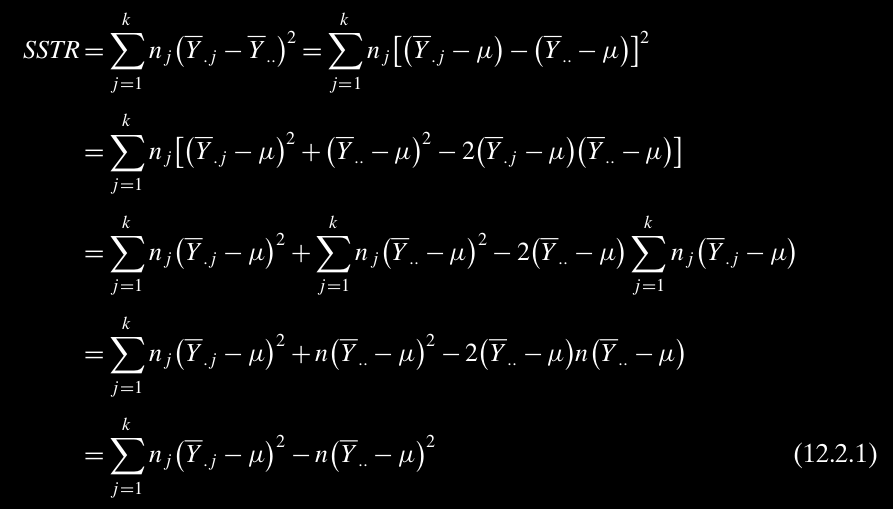
\includegraphics[scale=0.3]{Eq_12-2-1-neg.png}
	\end{center}
	\[\Downarrow\]
	\[
		SSTR = \sum_{j=1}^k n_j\left[\left(\overline{Y}_{\cdot j}-\mu_j \right)^2 - 2 \left(\overline{Y}_{\cdot j}-\mu_j \right) \left(\mu-\mu_j \right)+ \left(\mu-\mu_j \right)^2\right ]	-n  \left(\overline{Y}_{\cdot \cdot}-\mu \right)^2
	\]
\end{frame}
%-------------- end slide -------------------------------%}}}
%-------------- start slide -------------------------------%{{{ 12.24
\begin{frame}[fragile]

\begin{enumerate}
	\item[] Notice that \\[1em]
		\[
			\overline{Y}_{\cdot j}\sim N(\mu_j,\sigma^2/n_j)\qquad\text{and}\qquad
			\overline{Y}_{\cdot \cdot}\sim N(\mu,\sigma^2/n)
		\]
		\vfill
	\item[$\Longrightarrow$]
		\begin{align*}
			\E[SSTR]  =& \sum_{j=1}^k n_j \left[\frac{\sigma^2}{n_j} -2\times 0 + (\mu-\mu_j)^2\right]- n \frac{\sigma^2}{n}\\[1em]
			=& (k-1)\sigma^2 + \sum_{j=1}^k n_j (\mu-\mu_j)^2
		\end{align*}
		\vfill
	\item[Remark]
		\begin{enumerate}
			\item[] When $\mu_1=\cdots=\mu_j$ then \\[1em]
			\item $\E[SSTR]=(k-1)\sigma^2$  \\[1em]
			\item $MSTR:=\frac{SSTR}{k-1}$
				is an unbiased estimator for $\sigma^2$.\\[1em]
			\item $SSTR/\sigma^2 \sim$ Chi square $(df=k-1)$.\hfill (Homework)
		\end{enumerate}
\end{enumerate}
\end{frame}
%-------------- end slide -------------------------------%}}}
%-------------- start slide -------------------------------%{{{ 12.25
\begin{frame}[fragile]

	\begin{enumerate}
		\item[] Test $H_0:\mu_1=\cdots=\mu_k$ v.s. $\mu_j$ are not the same.
			\vfill
		\item[Case I.] when $\sigma^2$ is known.\\[2em]
		\item[] Reject $H_0$ if $SSTR/\sigma^2\ge \chi^2_{1-\alpha,k-1}$.
			\vfill
		\item[Case II.] when $\sigma^2$ is unknown.\\[2em]
		\item[] ......
	\end{enumerate}
\end{frame}
%-------------- end slide -------------------------------%}}}
%-------------- start slide -------------------------------%{{{ 12.26
\begin{frame}[fragile]{Sum of Squared Errors: SSE}

	\begin{enumerate}
		\item Sum of squred error:
			\vfill
	\begin{align*}
		SSE:=& \sum_{j=1}^k\sum_{i=1}^{n_j} \left(Y_{ij}-\overline{Y}_{\cdot j} \right)^2\\[1em]
		=& \sum_{j=1}^k(n_j-1)\left[ \frac{1}{n_j-1} \sum_{i=1}^{n_j} \left(Y_{ij}-\overline{Y}_{\cdot j} \right)^2\right]\\[1em]
		=&\sum_{j=1}^k(n_j-1) S_j^2
	\end{align*}
	\vfill
	\item Pooled variance $S_p^2$:
		\vfill
	\[
		S_p^2 = \frac{SSE}{\sum_{j=1}^k (n_j-1)} = \frac{SSE}{n-k}
	\]
\item[] Mean square of error $MSE = S_p^2$
	\end{enumerate}
\end{frame}
%-------------- end slide -------------------------------%}}}
%-------------- start slide -------------------------------%{{{ 12.27
\begin{frame}[fragile]


\begin{enumerate}
	\item[] Notice that\\[1em]
	\item $(n_j-1)S_j^2/\sigma^2\sim $Chi square $(df=n_j-1)$
	\item $S_j^2$'s are independent
	\item $SSE/\sigma^2 = (n-k) S_p^2/\sigma^2= \sum_{j=1}^k (n_j-1)S_j^2/\sigma^2 $,
	\item[] \qquad\qquad Sum of independent of Chi squares
		\[\Downarrow\]
	\item[Thm.] No mattter $H_0:\mu_1=\cdots=\mu_k$ is true or not
	\item[a.] $SSE/\sigma^2 = (n-k) S_p^2/\sigma^2\sim$ Chi square $(df=\sum_{j=1}^k(n_j-1) = n-k)$
	\item[b.] $SSTR \perp SSE$.
		\vfill
	\item[Proof.] We have shown part (a). Part (b) is trickier. Indeed, both parts are a consequence of \textcolor{yellow!80!black}{\bf Cochran's theorem}\footnote{\url{https://en.wikipedia.org/wiki/Cochran\%27s_theorem}} ... \myEnd
\end{enumerate}

\end{frame}
%-------------- end slide -------------------------------%}}}
%-------------- start slide -------------------------------%{{{ 12.28
\begin{frame}[fragile]

	\begin{enumerate}
		\item[] Let's see two special cases of
			\vfill
	\item[Thm.] No mattter $H_0:\mu_1=\cdots=\mu_k$ is true or not
	\item[a.] $SSE/\sigma^2 = (n-k) S_p^2/\sigma^2\sim$ Chi square $(df=\sum_{j=1}^k(n_j-1) = n-k)$
	\item[b.] $SSTR \perp SSE$.
		\vfill
	\item[Cases]
			\setcounter{enumi}{0}
		\item $k=1$, one sample case, $S_p^2$ is sample variance\hfill {\small Chapter 7}\\[0.6em]
		\item[] a. $(n-1)S^2/\sigma^2\sim \chi^2(n-1)$
		\item[] b. $SSTR\equiv 0$\\[1em]
		\item $k=2$, two sample case\hfill {\small Chapter 9}\\[0.6em]
		\item[] a. $(n-2)S_p^2/\sigma^2 \sim\chi^2(n-2)$
		\item[] b. $\overline{X}-\overline{Y}\perp S_p^2$ $\quad\Longleftrightarrow\quad$ $SSTR\perp SSE$
	\end{enumerate}
\end{frame}
%-------------- end slide -------------------------------%}}}
%-------------- start slide -------------------------------%{{{ 12.29
\begin{frame}[fragile]
Under $H_0: \mu_1=\cdots = \mu_k$
\begin{enumerate}
	\item $SSTR/\sigma^2 \sim \chi^2(k-1)$
	\item $SSE/\sigma^2 \sim \chi^2(n-k)$
	\item $SSTR\perp SSE$
		\vfill
	\item[$\Longrightarrow$] $\qquad \displaystyle F = \frac{SSTR/(k-1)}{SSE/(n-k)}\sim F(df_1=k-1,df_2=n-k)$
		\vfill
	\item[Reject] $H_0$ if $F\ge F_{1-\alpha,k-1,n-k}$
\end{enumerate}
\end{frame}
%-------------- end slide -------------------------------%}}}
%-------------- start slide -------------------------------%{{{ 12.30
\begin{frame}[fragile]{Total Sum of Squares: SSTOT\\[0.4em]
	SSTOT=SSE+SSTR}

	\[SSTOT:= \sum_{j=1}^k\sum_{i=1}^{n_j} \left(Y_{ij}-\overline{Y}_{\cdot \cdot} \right)^2
	\]
	\[||\]
	\begin{gather*}
		\sum_{j=1}^k\sum_{i=1}^{n_j}\left[ \left(Y_{ij}-\overline{Y}_{j \cdot} \right)+ \left(\overline{Y}_{\cdot j}-\overline{Y}_{\cdot \cdot} \right) \right]^2
 \\ ||\\
 \sum_{j=1}^k\sum_{i=1}^{n_j}\left(Y_{ij}-\overline{Y}_{j \cdot} \right)^2+2\sum_{j=1}^k\sum_{i=1}^{n_j}\left(Y_{ij}-\overline{Y}_{\cdot j} \right)\left(\overline{Y}_{\cdot j}-\overline{Y}_{\cdot \cdot} \right)+\sum_{j=1}^k\sum_{i=1}^{n_j}\left(\overline{Y}_{\cdot j}-\overline{Y}_{\cdot \cdot} \right)^2
 \\ ||\\
 \sum_{j=1}^k\sum_{i=1}^{n_j}\left(Y_{ij}-\overline{Y}_{j \cdot} \right)^2+2\sum_{j=1}^k\left(\overline{Y}_{\cdot j}-\overline{Y}_{\cdot \cdot} \right)\sum_{i=1}^{n_j}\left(Y_{ij}-\overline{Y}_{\cdot j} \right)+\sum_{j=1}^kn_j\left(\overline{Y}_{\cdot j}-\overline{Y}_{\cdot \cdot} \right)^2
 \\ ||\\
 SSE + 0 + SSTR
	\end{gather*}
\end{frame}
%-------------- end slide -------------------------------%}}}
%-------------- start slide -------------------------------%{{{ 12.31
\begin{frame}[fragile]
	\begin{center}
		\begin{tabular}{ccccc}
			$\displaystyle SSTOT$ &
			= &
			$\displaystyle SSE$ &
			+ &
			$\displaystyle SSTR$ \\ \\
			  &$\Downarrow$&&& \\ \\
			$\displaystyle \frac{SSTOT}{\sigma^2}$ &
			= &
			$\displaystyle \frac{SSE}{\sigma^2}$ &
			+ &
			$\displaystyle \frac{SSTR}{\sigma^2}$ \\ \\
			$\wr$&& $\wr$ &  & $\wr$ \\ \\
			$\chi^2(n-1)$ && $\chi^2(n-k)$ & $\perp$ & $\chi^2(k-1)$
			\\[2em]
			Under $H_0$& & \checkmark && Under $H_0$
		\end{tabular}
	\end{center}
\end{frame}
%-------------- end slide -------------------------------%}}}
%-------------- start slide -------------------------------%{{{ 12.32
\begin{frame}
	\centering
	% 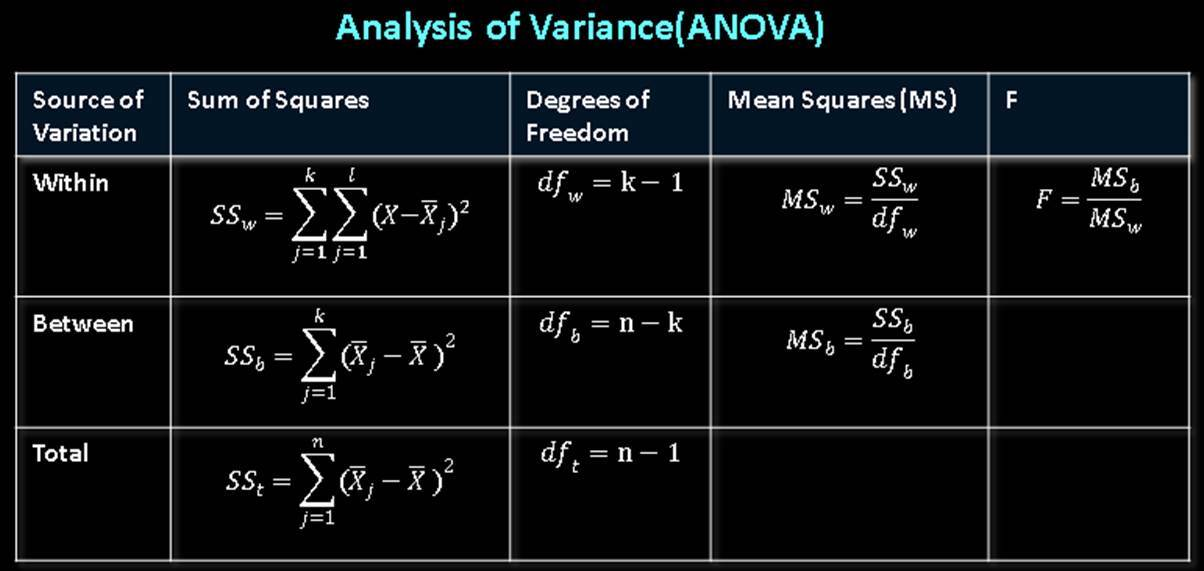
\includegraphics[scale=0.4]{Anova_Table-neg.jpg}
	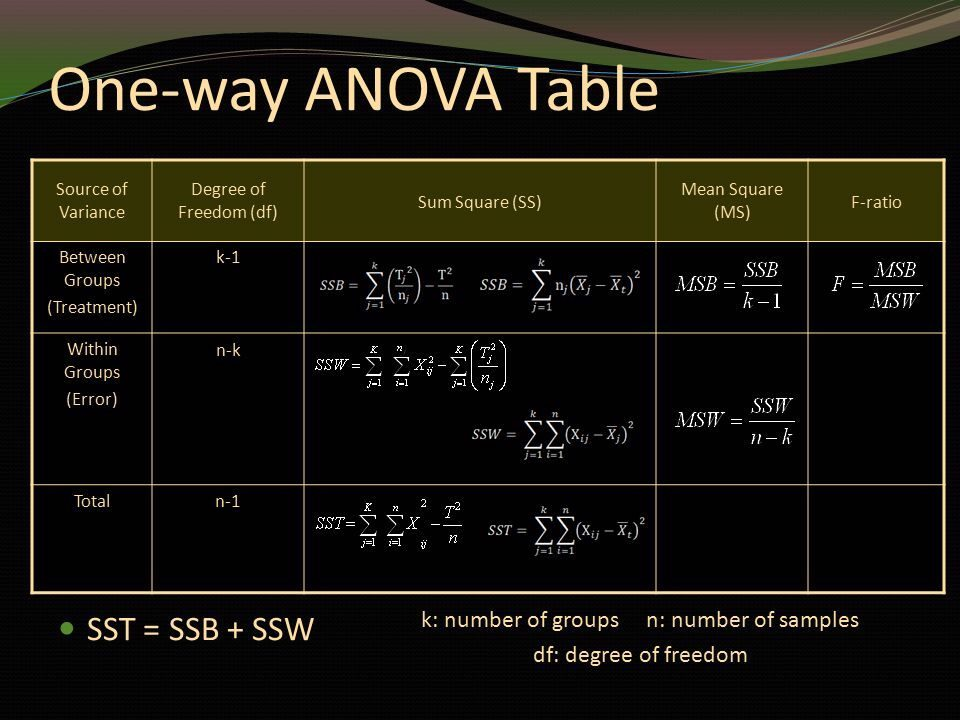
\includegraphics[scale=0.25]{Anova_Table3-neg.jpg}
	\vfill
	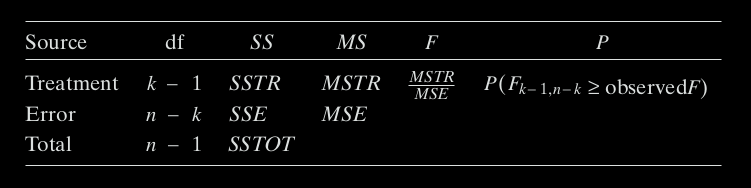
\includegraphics[scale=0.3]{Figure_12-2-1-neg.png}
\end{frame}
%-------------- end slide -------------------------------%}}}
%-------------- start slide -------------------------------%{{{ 12.33
\begin{frame}{Common notation}

\begin{enumerate}
	\item[d.f.\hspace{1.2em}]\phantom{a}\\[2em]
	\item[k-1\hspace{1.2em}]  Error sum of squares \hfill $SSE = SSW = SS_{within}$
	\item[] Mean square of error\hfill $MSE=MSW=MS_{within}=S_p^2$
	\item[] (Pooled sample variance)
		\vfill
	\item[n-k\hspace{1.2em}] Treatment sum of squares \hfill $SSTR = SSB = SS_{between}$
	\item[] Mean square of treatment\hfill $MSTR = MSB=MS_{between}$
		\vfill
	\item[n-1\hspace{1.2em}] Total sum of squares:\hfill $SST = SSTOT$
\end{enumerate}
\end{frame}
%-------------- end slide -------------------------------%}}}
%-------------- start slide -------------------------------%{{{ 12.34
\begin{frame}[fragile]{One way ANOVA v.s. Two sample $t$-test}
\begin{enumerate}
	\item[] Let $X_1,\cdots, X_n$ and $Y_1,\cdots, Y_m$ be samples from $N(\mu_X,\sigma^2)$ and $N(\mu_Y,\sigma^2)$, respectively.
		\vfill
	\item[Recall]
	\item $\displaystyle SSTR/\sigma^2 = \frac{\left(\overline{X}-\overline{Y}\right)^2}{\sigma^2\left(\frac 1n+\frac 1m\right)}\hspace{4em}\sim \chi^2(1)$
	\item $SSE/\sigma^2 = (n+m-2)S_p^2/\sigma^2\hspace{2em}\sim\chi^2(n+m-2)$
		\vfill
	\item[$\Longrightarrow$] $\displaystyle F= \frac{SSTR/1}{SSE/(n+m-2)}=\frac{\left(\overline{X}-\overline{Y}\right)^2}{S_p^2\left(\frac 1n+\frac 1m\right)} $ $\sim F(df_1=1,df_2=n+m-2)$
	\item[] \hspace{14em}$||$
	\item[] \hspace{14em}$T^2$
		\vfill
\item[$\Longrightarrow$]
		$\alpha = \bbP\left(|T|\ge t_{\alpha/2,n+m-2} \right )
		= \bbP\left(T^2\ge t_{\alpha/2,n+m-2}^2 \right )
		=  \bbP\left( F \ge F_{1-\alpha,1,n+m-2} \right)$
\item[]\phantom{a}
	\begin{center}
	Equivalent!
	\end{center}
\end{enumerate}
\end{frame}
%-------------- end slide -------------------------------%}}}
%-------------- start slide -------------------------------%{{{ 12.35
\begin{frame}
	\begin{enumerate}
		\item[E.g. 1] Study the relation between smoking and heart rates.\\[1em]
Generations of athletes have been cautioned that cigarette smoking impedes
performance. One measure of the truth of that warning is the effect of smoking
on heart rate. In one study, six nonsmokers, six light smokers, six moderate
smokers, and six heavy smokers each engaged in sustained physical exercise.
Table 8.1.1 lists their heart rates after they had rested for three minutes.
\\[1em]
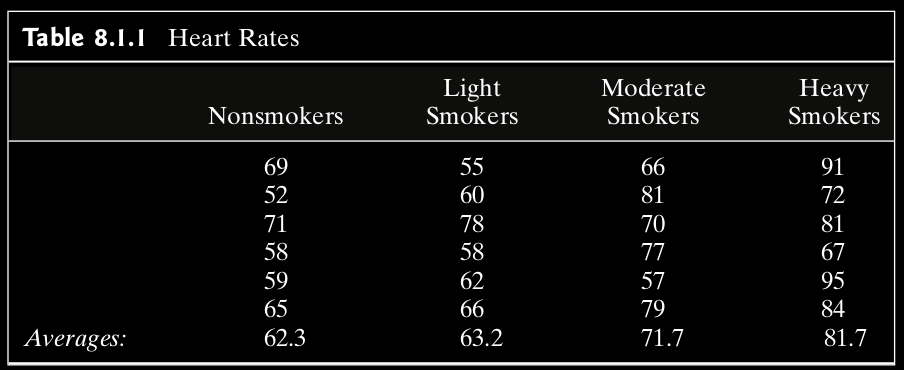
\includegraphics[scale=0.25]{Table_8-1-1-neg.png}
\item[] Show whether smoking affects heart rates at $\alpha=0.05$.
	\end{enumerate}
\end{frame}
%-------------- end slide -------------------------------%}}}
%-------------- start slide -------------------------------%{{{ 12.36
\begin{frame}

	\begin{enumerate}
		\item[Sol.] Let $\mu_1,\cdots,\mu_4$ be the true heart rates.
			\vfill
		\item[] Test $H_0:\mu_0= \cdots = \mu_4$ or not.
			\vfill
		\item[] Critical region:\\
			\vfill
			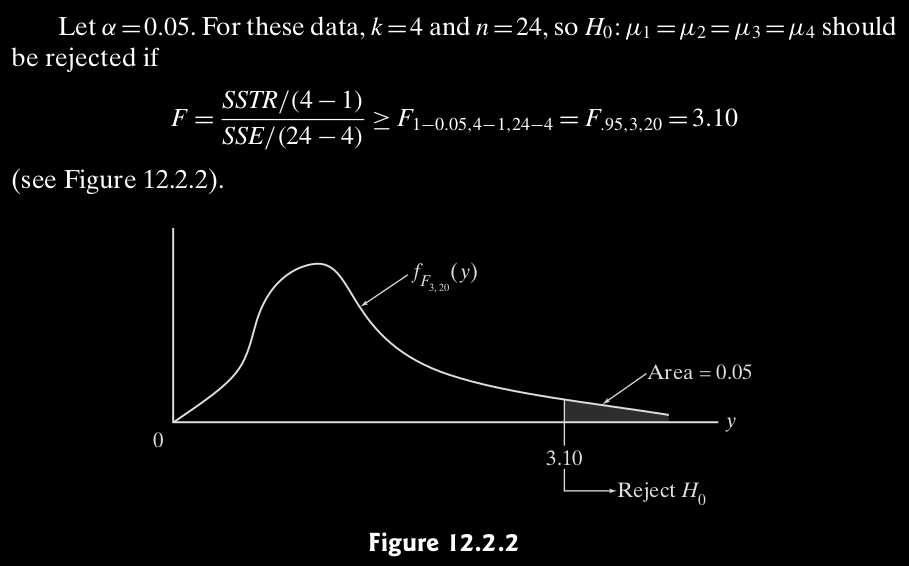
\includegraphics[scale=0.3]{Figure_12-2-2-neg.png}
	\end{enumerate}
\end{frame}
%-------------- end slide -------------------------------%}}}
%-------------- start slide -------------------------------%{{{ 12.37
\begin{frame}
\centering
	\begin{enumerate}
		\item[]  Computing....
			\vfill
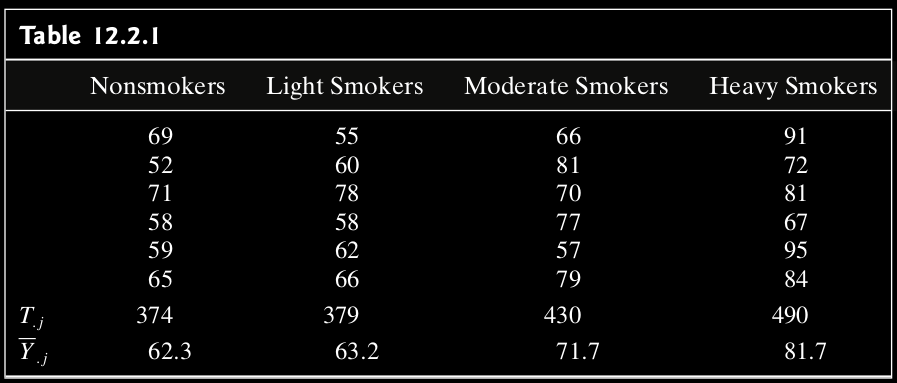
\includegraphics[scale=0.25]{Table_12-2-1-neg.png}	\\
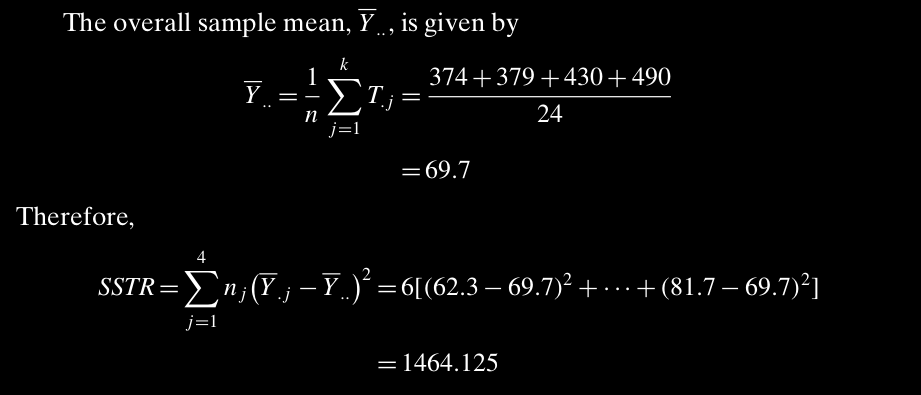
\includegraphics[scale=0.25]{Case_12-2-1-1-neg.png}\\
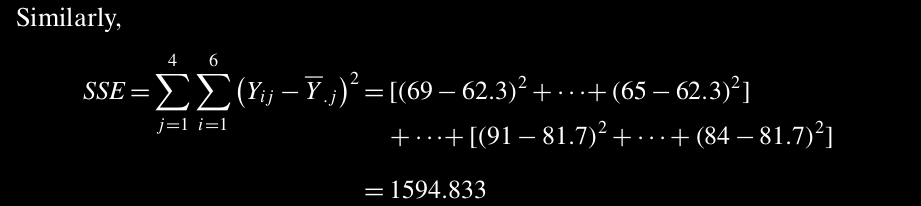
\includegraphics[scale=0.25]{Case_12-2-1-2-neg.png}
	\end{enumerate}
\end{frame}
%-------------- end slide -------------------------------%}}}
%-------------- start slide -------------------------------%{{{ 12.38
\begin{frame}
	\centering
	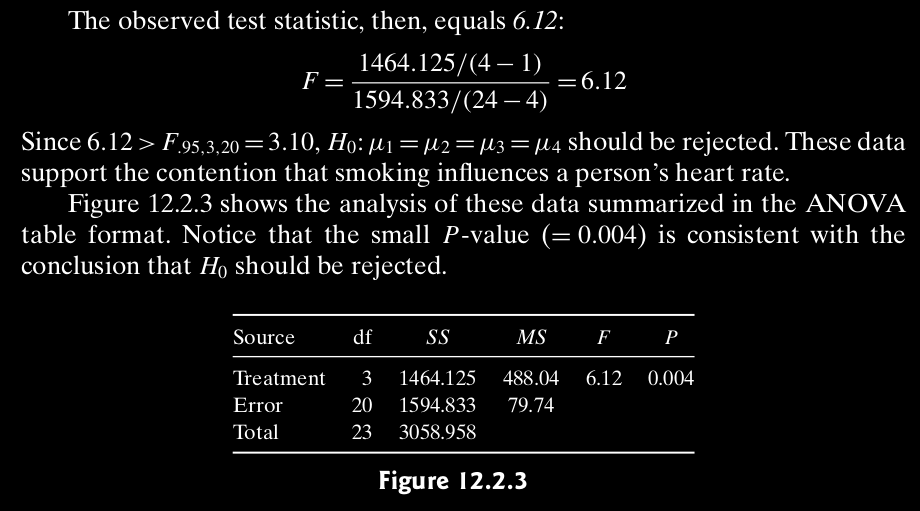
\includegraphics[scale=0.3]{Figure_12-2-3-neg.png}
	\myEnd
\end{frame}
%-------------- end slide -------------------------------%}}}
%-------------- start slide -------------------------------%{{{ 12.39
\begin{frame}[fragile]{\small\url{http://www.sthda.com/english/wiki/one-way-anova-test-in-r}}
	\begin{minipage}{0.45\textwidth}
	\begin{lstlisting}
> Input <-c("
+ rates group
+ 69  non
+ 52  non
+ 71  non
+ 58  non
+ 59  non
+ 65  non
+ 55  light
+ 60  light
+ 78  light
+ 58  light
+ 62  light
+ 66  light
+ 66  moderate
+ 81  moderate
+ 70  moderate
+ 77  moderate
+ 57  moderate
+ 79  moderate
+ 91  heavy
+ 72  heavy
+ 81  heavy
+ 67  heavy
+ 95  heavy
+ 84  heavy
+ ")
> Data = read.table(textConnection(Input),
+                   header=TRUE)
	\end{lstlisting}
	\end{minipage}
	\hfill
	\begin{minipage}{0.45\textwidth}
	\begin{lstlisting}
> Data
   rates    group
1     69      non
2     52      non
3     71      non
4     58      non
5     59      non
6     65      non
7     55    light
8     60    light
9     78    light
10    58    light
11    62    light
12    66    light
13    66 moderate
14    81 moderate
15    70 moderate
16    77 moderate
17    57 moderate
18    79 moderate
19    91    heavy
20    72    heavy
21    81    heavy
22    67    heavy
23    95    heavy
24    84    heavy
	\end{lstlisting}
	\end{minipage}
\end{frame}
%-------------- end slide -------------------------------%}}}
%-------------- start slide -------------------------------%{{{ 12.40
\begin{frame}[fragile]
	\begin{center}
	\begin{lstlisting}
> # Check the levels
> levels(Data$group)
[1] "heavy"    "light"    "moderate" "non"
> # Order the groups
> Data$group <- ordered(Data$group, levels = c("non", "light","moderate", "heavy"))
> levels(Data$group)
[1] "non"      "light"    "moderate" "heavy"
	\end{lstlisting}
	\vfill
	\begin{lstlisting}
> # Compute summary statistics by groups
> # including count, mean, sd:
> library(dplyr) # a grammar of data manipulation
> group_by(Data, group) %>%
+   summarise(
+     count = n(),
+     mean = mean(rates, na.rm = TRUE),
+     sd = sd(rates, na.rm = TRUE)
+   )
# A tibble: 4 x 4
  group    count  mean    sd
  <ord>    <int> <dbl> <dbl>
1 non          6  62.3  7.26
2 light        6  63.2  8.16
3 moderate     6  71.7  9.16
4 heavy        6  81.7 10.8
	\end{lstlisting}
	\end{center}
\end{frame}
%-------------- end slide -------------------------------%}}}
%-------------- start slide -------------------------------%{{{ 12.41
\begin{frame}[fragile]
	\begin{center}
	\begin{lstlisting}
# Box plots
# ++++++++++++++++++++
# Plot rates by group and color by group
library(ggpubr)
png("Case_12-2-1-ggboxplot.png")
ggboxplot(Data, x = "group", y = "rates",
          color = "group", palette = c("#00AFBB", "#E7B800", "#FC4E07", "blue"),
          order = c("non", "light", "moderate","heavy"),
          ylab = "Rates", xlab = "Treatment")
dev.off()
	\end{lstlisting}
	\vfill
	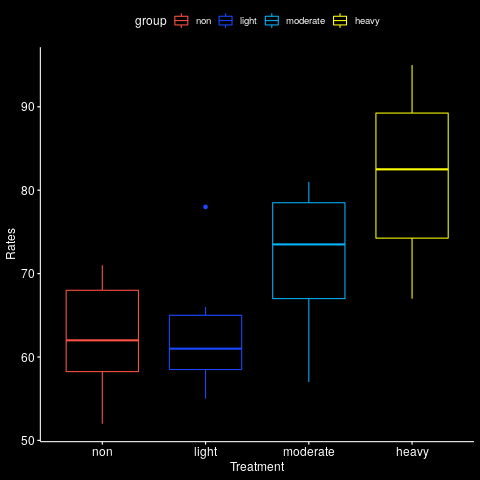
\includegraphics[scale=0.25]{Case_12-2-1-ggboxplot-neg.png}
	\end{center}
\end{frame}
%-------------- end slide -------------------------------%}}}
%-------------- start slide -------------------------------%{{{ 12.42
\begin{frame}[fragile]
	\begin{center}
	\begin{lstlisting}
# Mean plots
# ++++++++++++++++++++
# Plot rates by group
# Add error bars: mean_se
# (other values include: mean_sd, mean_ci, median_iqr, ....)
png("Case_12-2-1-ggline.png")
library(ggpubr)
ggline(Data, x = "group", y = "rates",
       add = c("mean_se", "jitter"),
       order =  c("non", "light", "moderate","heavy"),
       ylab = "Rates", xlab = "Treatment")
dev.off()
	\end{lstlisting}
	\vfill
	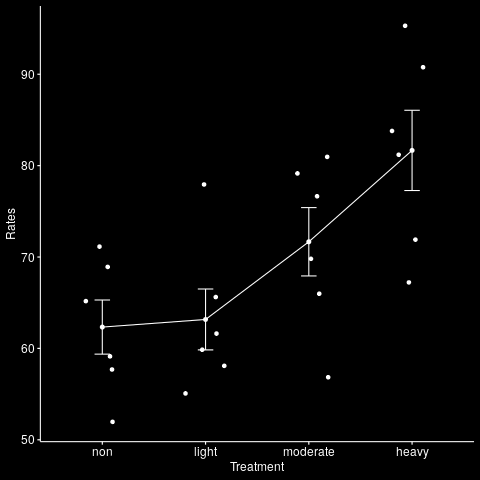
\includegraphics[scale=0.25]{Case_12-2-1-ggline-neg.png}
	\end{center}
\end{frame}
%-------------- end slide -------------------------------%}}}
%-------------- start slide -------------------------------%{{{ 12.43
\begin{frame}[fragile]
\begin{lstlisting}
> # Compute the analysis of variance
> res.aov <- aov(rates ~ group, data = Data)
> # Summary of the analysis
> summary(res.aov)
            Df Sum Sq Mean Sq F value  Pr(>F)
group        3   1464   488.0    6.12 0.00398 **
Residuals   20   1595    79.7
---
Signif. codes:  0 '***' 0.001 '**' 0.01 '*' 0.05 '.' 0.1 ' ' 1
\end{lstlisting}
\end{frame}
%-------------- end slide -------------------------------%}}}
%-------------- start slide -------------------------------%{{{ 12.44
\begin{frame}[fragile]
\begin{lstlisting}
> # Tukey multiple multiple-comparisons
> TukeyHSD(res.aov)
  Tukey multiple comparisons of means
    95% family-wise confidence level

Fit: aov(formula = rates ~ group, data = Data)

$group
                     diff        lwr      upr     p adj
light-non       0.8333333 -13.596955 15.26362 0.9984448
moderate-non    9.3333333  -5.096955 23.76362 0.2978123
heavy-non      19.3333333   4.903045 33.76362 0.0063659
moderate-light  8.5000000  -5.930289 22.93029 0.3755571
heavy-light    18.5000000   4.069711 32.93029 0.0091463
heavy-moderate 10.0000000  -4.430289 24.43029 0.2438158
\end{lstlisting}
\vfill
\begin{enumerate}
	\item diff: difference between means of the two groups
	\item lwr, upr: the lower and the upper end point of the C.I. at 95\% (default)
	\item p adj: p-value after adjustment for the multiple comparisons
		\vspace{1em}
	\item[]
		\begin{center}
			Inferences \\
		if p-value $\le 0.05$  $\quad\Longleftrightarrow\quad$ if zero is in the C.I.
		\end{center}
\end{enumerate}
\end{frame}
%-------------- end slide -------------------------------%}}}
%-------------- start slide -------------------------------%{{{ 12.45
\begin{frame}[fragile]
\begin{lstlisting}
> # Or one may use multcomp package or multiple comparisons
> library(multcomp)
> summary(glht(res.aov, linfct = mcp(group = "Tukey")))

	 Simultaneous Tests for General Linear Hypotheses

Multiple Comparisons of Means: Tukey Contrasts


Fit: aov(formula = rates ~ group, data = Data)

Linear Hypotheses:
                      Estimate Std. Error t value Pr(>|t|)
light - non == 0        0.8333     5.1556   0.162  0.99844
moderate - non == 0     9.3333     5.1556   1.810  0.29776
heavy - non == 0       19.3333     5.1556   3.750  0.00629 **
moderate - light == 0   8.5000     5.1556   1.649  0.37544
heavy - light == 0     18.5000     5.1556   3.588  0.00901 **
heavy - moderate == 0  10.0000     5.1556   1.940  0.24382
---
Signif. codes:  0 '***' 0.001 '**' 0.01 '*' 0.05 '.' 0.1 ' ' 1
(Adjusted p values reported -- single-step method)
\end{lstlisting}
\end{frame}
%-------------- end slide -------------------------------%}}}
%-------------- start slide -------------------------------%{{{ 12.46
\begin{frame}[fragile]
\begin{center}
\begin{lstlisting}
# Check ANOVA assumptions: test validity?
# diagnostic plots
layout(matrix(c(1,2),1,2)) # optional 1x2 graphs/page
plot(res.aov,c(1,2))
\end{lstlisting}
\vfill
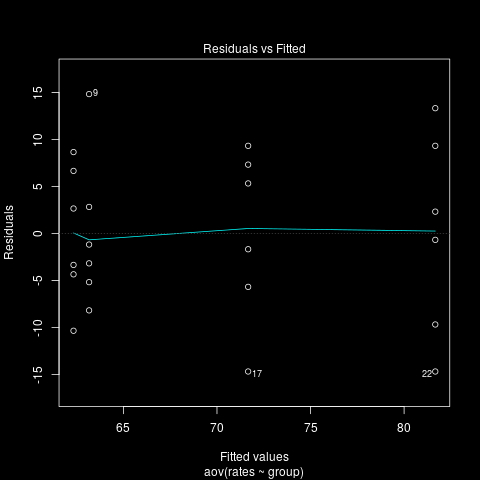
\includegraphics[scale=0.3]{Case_12-2-1-diagnostic_plots1-neg.png}
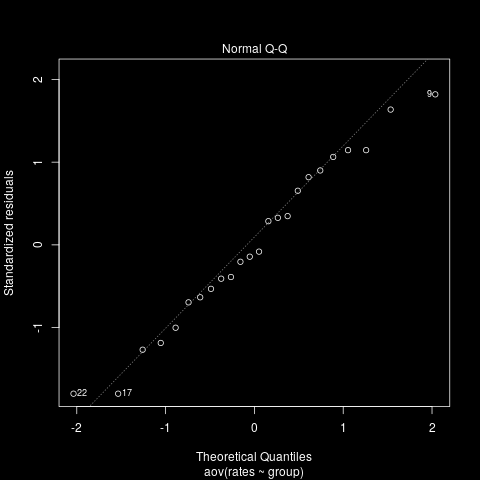
\includegraphics[scale=0.3]{Case_12-2-1-diagnostic_plots2-neg.png}
\end{center}
\end{frame}
%-------------- end slide -------------------------------%}}}
%-------------- start slide -------------------------------%{{{ 12.47
\begin{frame}[fragile]

	\begin{enumerate}
		\item Residuals vs Fitted: test homogeneity of variances\\
			One can also use Levene's test for this purpose:
		\item[]
			\begin{minipage}{0.7\textwidth}
\begin{lstlisting}
> # Use Levene's test to gest homogeneity of variances
> library(car)
> leveneTest(rates ~ group, data = Data)
Levene's Test for Homogeneity of Variance (center = median)
      Df F value Pr(>F)
group  3  0.3885 0.7625
      20
\end{lstlisting}
			\end{minipage}
\vfill
\item Normal Q-Q plot: Test normality. (It should be close to diagonal line.)\\
One can also use Shapiro-Wilk test:
\item[]
	\begin{minipage}{0.70\textwidth}
\begin{lstlisting}
# Extract the residuals
> aov_residuals <- residuals(object = res.aov )
> # Run Shapiro-Wilk test
> shapiro.test(x = aov_residuals )

	Shapiro-Wilk normality test

data:  aov_residuals
W = 0.9741, p-value = 0.7677
\end{lstlisting}
	\end{minipage}
	\end{enumerate}
\end{frame}
%-------------- end slide -------------------------------%}}}
%-------------- start slide -------------------------------%{{{ 12.48
\begin{frame}[fragile]{Non-parametric alternative to one-way ANOVA test}
	\begin{center}
	\begin{minipage}{0.7\textwidth}
\begin{lstlisting}
> # Non-parametric alternative to one-way ANOVA test
> # a non-parametric alternative to one-way ANOVA
> # is Kruskal-Wallis rank sum test, which can be
> # used when ANNOVA assumptions are not met.
> kruskal.test(rates ~ group, data = Data)

	Kruskal-Wallis rank sum test

data:  rates by group
Kruskal-Wallis chi-squared = 10.729, df = 3, p-value = 0.01329
\end{lstlisting}
	\end{minipage}
\vfill
{\small
	See Section 4 of Chapter 14 for more details.}
\end{center}
\end{frame}
%-------------- end slide -------------------------------%}}}
